\documentclass[12pt,letterpaper,fleqn]{hmcpset}
\usepackage[margin=1in]{geometry}
\usepackage{graphicx}
\usepackage{amsmath,amssymb}
\usepackage{enumerate}
\usepackage{hyperref}
\usepackage{parskip}
\usepackage{listings}

% Theorems
\usepackage{amsthm}
\renewcommand\qedsymbol{$\blacksquare$}
\makeatletter
\@ifclassloaded{article}{
    \newtheorem{definition}{Definition}[section]
    \newtheorem{example}{Example}[section]
    \newtheorem{theorem}{Theorem}[section]
    \newtheorem{corollary}{Corollary}[theorem]
    \newtheorem{lemma}{Lemma}[theorem]
}{
}
\makeatother

% Random Stuff
\setlength\unitlength{1mm}

\newcommand{\insertfig}[3]{
\begin{figure}[htbp]\begin{center}\begin{picture}(120,90)
\put(0,-5){\includegraphics[width=12cm,height=9cm,clip=]{#1.eps}}\end{picture}\end{center}
\caption{#2}\label{#3}\end{figure}}

\newcommand{\insertxfig}[4]{
\begin{figure}[htbp]
\begin{center}
\leavevmode \centerline{\resizebox{#4\textwidth}{!}{\input
#1.pstex_t}}
\caption{#2} \label{#3}
\end{center}
\end{figure}}

\long\def\comment#1{}

\newcommand\norm[1]{\left\lVert#1\right\rVert}
\DeclareMathOperator*{\argmin}{arg\,min}
\DeclareMathOperator*{\argmax}{arg\,max}

% bb font symbols
\newfont{\bbb}{msbm10 scaled 700}
\newcommand{\CCC}{\mbox{\bbb C}}

\newfont{\bbf}{msbm10 scaled 1100}
\newcommand{\CC}{\mbox{\bbf C}}
\newcommand{\PP}{\mbox{\bbf P}}
\newcommand{\RR}{\mbox{\bbf R}}
\newcommand{\QQ}{\mbox{\bbf Q}}
\newcommand{\ZZ}{\mbox{\bbf Z}}
\renewcommand{\SS}{\mbox{\bbf S}}
\newcommand{\FF}{\mbox{\bbf F}}
\newcommand{\GG}{\mbox{\bbf G}}
\newcommand{\EE}{\mbox{\bbf E}}
\newcommand{\NN}{\mbox{\bbf N}}
\newcommand{\KK}{\mbox{\bbf K}}
\newcommand{\KL}{\mbox{\bbf KL}}

% Vectors
\renewcommand{\aa}{{\bf a}}
\newcommand{\bb}{{\bf b}}
\newcommand{\cc}{{\bf c}}
\newcommand{\dd}{{\bf d}}
\newcommand{\ee}{{\bf e}}
\newcommand{\ff}{{\bf f}}
\renewcommand{\gg}{{\bf g}}
\newcommand{\hh}{{\bf h}}
\newcommand{\ii}{{\bf i}}
\newcommand{\jj}{{\bf j}}
\newcommand{\kk}{{\bf k}}
\renewcommand{\ll}{{\bf l}}
\newcommand{\mm}{{\bf m}}
\newcommand{\nn}{{\bf n}}
\newcommand{\oo}{{\bf o}}
\newcommand{\pp}{{\bf p}}
\newcommand{\qq}{{\bf q}}
\newcommand{\rr}{{\bf r}}
\renewcommand{\ss}{{\bf s}}
\renewcommand{\tt}{{\bf t}}
\newcommand{\uu}{{\bf u}}
\newcommand{\ww}{{\bf w}}
\newcommand{\vv}{{\bf v}}
\newcommand{\xx}{{\bf x}}
\newcommand{\yy}{{\bf y}}
\newcommand{\zz}{{\bf z}}
\newcommand{\0}{{\bf 0}}
\newcommand{\1}{{\bf 1}}

% Matrices
\newcommand{\Ab}{{\bf A}}
\newcommand{\Bb}{{\bf B}}
\newcommand{\Cb}{{\bf C}}
\newcommand{\Db}{{\bf D}}
\newcommand{\Eb}{{\bf E}}
\newcommand{\Fb}{{\bf F}}
\newcommand{\Gb}{{\bf G}}
\newcommand{\Hb}{{\bf H}}
\newcommand{\Ib}{{\bf I}}
\newcommand{\Jb}{{\bf J}}
\newcommand{\Kb}{{\bf K}}
\newcommand{\Lb}{{\bf L}}
\newcommand{\Mb}{{\bf M}}
\newcommand{\Nb}{{\bf N}}
\newcommand{\Ob}{{\bf O}}
\newcommand{\Pb}{{\bf P}}
\newcommand{\Qb}{{\bf Q}}
\newcommand{\Rb}{{\bf R}}
\newcommand{\Sb}{{\bf S}}
\newcommand{\Tb}{{\bf T}}
\newcommand{\Ub}{{\bf U}}
\newcommand{\Wb}{{\bf W}}
\newcommand{\Vb}{{\bf V}}
\newcommand{\Xb}{{\bf X}}
\newcommand{\Yb}{{\bf Y}}
\newcommand{\Zb}{{\bf Z}}

% Calligraphic
\newcommand{\Ac}{{\cal A}}
\newcommand{\Bc}{{\cal B}}
\newcommand{\Cc}{{\cal C}}
\newcommand{\Dc}{{\cal D}}
\newcommand{\Ec}{{\cal E}}
\newcommand{\Fc}{{\cal F}}
\newcommand{\Gc}{{\cal G}}
\newcommand{\Hc}{{\cal H}}
\newcommand{\Ic}{{\cal I}}
\newcommand{\Jc}{{\cal J}}
\newcommand{\Kc}{{\cal K}}
\newcommand{\Lc}{{\cal L}}
\newcommand{\Mc}{{\cal M}}
\newcommand{\Nc}{{\cal N}}
\newcommand{\Oc}{{\cal O}}
\newcommand{\Pc}{{\cal P}}
\newcommand{\Qc}{{\cal Q}}
\newcommand{\Rc}{{\cal R}}
\newcommand{\Sc}{{\cal S}}
\newcommand{\Tc}{{\cal T}}
\newcommand{\Uc}{{\cal U}}
\newcommand{\Wc}{{\cal W}}
\newcommand{\Vc}{{\cal V}}
\newcommand{\Xc}{{\cal X}}
\newcommand{\Yc}{{\cal Y}}
\newcommand{\Zc}{{\cal Z}}

% Bold greek letters
\newcommand{\alphab}{\hbox{\boldmath$\alpha$}}
\newcommand{\betab}{\hbox{\boldmath$\beta$}}
\newcommand{\gammab}{\hbox{\boldmath$\gamma$}}
\newcommand{\deltab}{\hbox{\boldmath$\delta$}}
\newcommand{\etab}{\hbox{\boldmath$\eta$}}
\newcommand{\lambdab}{\hbox{\boldmath$\lambda$}}
\newcommand{\epsilonb}{\hbox{\boldmath$\epsilon$}}
\newcommand{\nub}{\hbox{\boldmath$\nu$}}
\newcommand{\mub}{\hbox{\boldmath$\mu$}}
\newcommand{\zetab}{\hbox{\boldmath$\zeta$}}
\newcommand{\phib}{\hbox{\boldmath$\phi$}}
\newcommand{\psib}{\hbox{\boldmath$\psi$}}
\newcommand{\thetab}{\hbox{\boldmath$\theta$}}
\newcommand{\taub}{\hbox{\boldmath$\tau$}}
\newcommand{\omegab}{\hbox{\boldmath$\omega$}}
\newcommand{\xib}{\hbox{\boldmath$\xi$}}
\newcommand{\sigmab}{\hbox{\boldmath$\sigma$}}
\newcommand{\pib}{\hbox{\boldmath$\pi$}}
\newcommand{\rhob}{\hbox{\boldmath$\rho$}}

\newcommand{\Gammab}{\hbox{\boldmath$\Gamma$}}
\newcommand{\Lambdab}{\hbox{\boldmath$\Lambda$}}
\newcommand{\Deltab}{\hbox{\boldmath$\Delta$}}
\newcommand{\Sigmab}{\hbox{\boldmath$\Sigma$}}
\newcommand{\Phib}{\hbox{\boldmath$\Phi$}}
\newcommand{\Pib}{\hbox{\boldmath$\Pi$}}
\newcommand{\Psib}{\hbox{\boldmath$\Psi$}}
\newcommand{\Thetab}{\hbox{\boldmath$\Theta$}}
\newcommand{\Omegab}{\hbox{\boldmath$\Omega$}}
\newcommand{\Xib}{\hbox{\boldmath$\Xi$}}

% mixed symbols
\newcommand{\sinc}{{\hbox{sinc}}}
\newcommand{\diag}{{\hbox{diag}}}
\renewcommand{\det}{{\hbox{det}}}
\newcommand{\trace}{{\hbox{tr}}}
\newcommand{\tr}{\trace}
\newcommand{\sign}{{\hbox{sign}}}
\renewcommand{\arg}{{\hbox{arg}}}
\newcommand{\var}{{\hbox{var}}}
\newcommand{\cov}{{\hbox{cov}}}
\renewcommand{\Re}{{\rm Re}}
\renewcommand{\Im}{{\rm Im}}
\newcommand{\eqdef}{\stackrel{\Delta}{=}}
\newcommand{\defines}{{\,\,\stackrel{\scriptscriptstyle \bigtriangleup}{=}\,\,}}
\newcommand{\<}{\left\langle}
\renewcommand{\>}{\right\rangle}
\newcommand{\Psf}{{\sf P}}
\newcommand{\T}{\top}
\newcommand{\m}[1]{\begin{bmatrix} #1 \end{bmatrix}}

% info for header block in upper right hand corner
\name{Nathaniel Diamant}
\class{Math 189r}
\assignment{Homework 3}
\duedate{November 7, 2016}

\begin{document}

There are 5 problems in this set. You need to do 3 problems the first week and 2 the second
week. Instead of a sixth problem, youare encouraged to work on your final project.
Feel free to work with other students, but make sure you write up the homework
and code on your own (no copying homework \textit{or} code; no pair programming).
Feel free to ask students or instructors for help debugging code or whatever else,
though.
When implementing algorithms you may not use any library (such as \texttt{sklearn})
that already implements the algorithms but you may use any other library for
data cleaning and numeric purposes (\texttt{numpy} or \texttt{pandas}). Use common
sense. Problems are in no specific order.\\[1em]

\textbf{1 (Murphy 11.2 - EM for Mixtures of Gaussians)} Show that the M step for ML
estimation of a mixture of Gaussians is given by
\begin{align*}
    \mub_k &= \frac{\sum_i r_{ik}\xx_i}{r_k}\\
    \Sigmab_k &= \frac{1}{r_k}\sum_i r_{ik}(\xx_i - \mub_k)(\xx_i - \mub_k)^\T = \frac{1}{r_k}\sum_i r_{ik}\xx_i\xx_i^\T - r_k\mub_k\mub_k^\T.
\end{align*}
\vspace{15mm}
We have that the log likelihood is $$ -\frac{1}{2} \sum_i r_{ik} \left[ \log|\Sigma_k| + (\xx_i - \mub_k)^\T \Sigma_k^{-1} (\xx_i - \mub_k) \right] $$

To find the means, we take $\frac{\partial}{\partial \mub_k} l(\mub_k, \Sigma_k) = 0$.
\begin{align*}
	0 &= \frac{\partial}{\partial \mub_k} -\frac{1}{2} \sum_i r_{ik} \left[ \log|\Sigma_k| + (\xx_i - \mub_k)^\T \Sigma_k^{-1} (\xx_i - \mub_k) \right] \\
	0 &= -\frac{1}{2}  \sum_i r_{ik} \frac{\partial}{\partial \mub_k} (\xx_i - \mub_k)^\T \Sigma_k^{-1} (\xx_i - \mub_k) &\\
	0 &= \sum_i r_{ik} \Sigma_{k}^{-1} (\xx_i - \mub_k) \text{  Matrix cookbook 86}\\
    \Sigma_{k}^{-1} \mub_k \sum_i r_{ik} &= \sum_i r_{ik} \Sigma_{k}^{-1} \xx_i \\
    \mub_k &= \frac{\sum_i r_{ik}\xx_i}{r_k} \text{ Multiplied by $\Sigma_{k}$ on both sides. }
\end{align*} 
Where $r_k =\sum_i r_{ik} $.

To find $\Sigma_k$, we take $\frac{\partial}{\partial \Sigma_k} l(\mub_k, \Sigma_k) = 0$.

\begin{align*}
    0 &= \frac{\partial}{\partial \Sigma_k} -\frac{1}{2} \sum_i r_{ik} \left[ \log|\Sigma_k| + (\xx_i - \mub_k)^\T \Sigma_k^{-1} (\xx_i - \mub_k) \right]\\
    &= \sum_i r_{ik} \left[ \frac{\partial}{\partial \Sigma_k} \log|\Sigma_k| + \frac{\partial}{\partial \Sigma_k}(\xx_i - \mub_k)^\T \Sigma_k^{-1} (\xx_i - \mub_k) \right] \\
    &= \sum_i r_{ik} \left[ \frac{\partial}{\partial \Sigma_k} \log|\Sigma_k| + (\xx_i - \mub_k) (\xx_i - \mub_k)^\T \right] \text{ Matrix Cookbook 72} \\
    &= \sum_i r_{ik} \left[ -\Sigma_k + (\xx_i - \mub_k) (\xx_i - \mub_k)^\T \right] \text{ Math stack exchange} \\
    \Sigma_k \sum_i r_{ik} &= \sum_i r_{ik} (\xx_i - \mub_k) (\xx_i - \mub_k)^\T\\
    \Sigma_k &= \frac{ \sum_i r_{ik} (\xx_i - \mub_k) (\xx_i - \mub_k)^\T}{r_k} \text{ Desired form 1}\\
    &= \frac{1}{r_k} \sum_i r_{ik} \left[\xx_i\xx_i^\T  - \xx_i \mub_k ^\T - \mub_k \xx_i^\T + \mub_k\mub_k^\T \right] \\
    &= \frac{1}{r_k} \sum_i r_{ik} \left[\xx_i\xx_i^\T - \mub_k\mub_k^\T \right] \\
    &= \frac{1}{r_k} \sum_i r_{ik} \xx_i\xx_i^\T - \frac{1}{r_k} \sum_i r_{ik} \mub_k\mub_k^\T \\
    &= \frac{1}{r_k} \sum_i r_{ik} \xx_i\xx_i^\T - \frac{r_k}{r_k} \sum_i \mub_k\mub_k^\T \\
    &= \frac{1}{r_k} \sum_i r_{ik} \xx_i\xx_i^\T -  \sum_i \mub_k\mub_k^\T \text{ As desired.}
    \end{align*}

\newpage


\textbf{2 (Murphy 11.3 - EM for Mixtures of Bernoullis)} Show that the M step for ML estimation
of a mixture of Bernoullis is given by
\[
    \mu_{kj} = \frac{\sum_i r_{ik}x_{ij}}{\sum_i r_{ik}}.
\]
Show that the M step for MAP estimation of a mixture of Bernoullis with a $\beta(\alpha,\beta)$ prior
is given by
\[
    \mu_{kj} = \frac{\left(\sum_i r_{ik}x_{ij}\right) + \alpha - 1}{\left(\sum_i r_{ik}\right) + \alpha + \beta - 2}.
\]

\vspace{15mm}
a) We have that the likelihood is 
\begin{align*}
    l(\thetab_k) &= \sum_i r_{ik}\log p(\xx_i | \theta_k) \\
    &= \sum_i r_{ik} \sum_j x_{ij}\log\mu_k + (1-x_{ij})\log[1-\mu_{kj}] \\
\end{align*}
Now we take $\frac{\partial}{\partial \mu_{kj}} l = 0$
\begin{align*}
    0 &= \sum_i r_{ik} \frac{\partial}{\partial \mub_{kj}} \log\mu_k + (1-x_{ij})\log[1-\mu_{kj}\\
    &= \sum_i r_{ik} x_{ij}/\mu_{kj} - (1-x_{ij})/(1-\mu_{kj})\\
    &= \sum_i r_{ik} x_{ij}(1-\mu_{kj}) /(\mu_{kj}(1-\mu_{kj})) - \mu_{kj}(1-x_{ij})/((1-\mu_{kj})\mu_{kj}) \\
    &= \sum_i r_{ik} \frac{x_{ij} - \mu_{kj}}{(1-\mu_{kj})\mu_{kj}}\\
    &= \sum_i r_{ik} (x_{ij} - \mu_{kj}) \\
    \mu_{jk} &= \frac{\sum_i r_{ik}x_{ij}}{r_k}
\end{align*}

Now we add a $\log p(\mu_k) = \sum_i \log \beta(\alpha, \beta)^{-1} \mu_{kj}^{\alpha -1} (1-\mu_{kj})$ term to the MLE. Now when we take $\frac{\partial}{\partial \mu_{kj}} l = 0$, we get,
\begin{align*}
    0 &= \sum_i r_{ik}x_{ij}/ \mu_{kj} + (1-x{kj})/(1-\mu_{kj}) + (\alpha -1) / \mu_{kj} + (\beta - 1) / (1-\mu_kj) \\
    &= \sum_{i} r_{ik}x_{ij} + \alpha -1 - \mu_{kj}r_{ik}x_{ij} + \mu_{kj}\alpha - \mu_{kj} - \mu_{kj}r_{ik} + \mu_{kj}x_{ij} - \mu_{kj} \beta + \mu_{kj} \\
    & \text{(Pulled out common denominator)} \\
    &= \sum_i r_{ik}x_{ij} + \alpha -1 - \mu_{kj} (r_{ik} + \alpha + \beta - 2)\\
    \mu_{kj} &= \frac{\sum_i \left[ r_{ik}x_{ij} + \alpha -1 \right]}{\sum_i [r_{ik} + \alpha + \beta -2]}
\end{align*}
Note: the math almost worked out. Not quite sure why $\alpha, \beta, -2$ are not in the sum.

\newpage

\textbf{3 (MAP Mixture of Gaussians)} Consider a mixture of Gaussians with a Dirichlet prior on the
mixture weights $\pib \sim \mathrm{Dir}(\alphab)$ and a Negative Inverse Walshart prior on the
mean and covariance within each class
$\mub_k,\Sigmab_k \sim \mathrm{NIW}(\mathbf{m}_0,\kappa_0,\nu_0,\mathbf{S}_0)$ with $\kappa_0=0$ so
only the covariance matrices are regularized. Use $\mathbf{S}_0 = \mathrm{diag}(s_1^2,\dots,s_D^2)/K^{1/D}$
where $s_j = \sum_i(x_{ij} - \overline{x}_j)^2/N$ is the pooled variance in dimension $j$. Use $\nu_0 = D + 2$,
as that is the weakest prior that is still proper. Use $\alphab = \1$. This is all detailed in Murphy 11.4.2.8. Download the
wine quality data at \url{https://archive.ics.uci.edu/ml/machine-learning-databases/wine-quality/winequality-red.csv}
and \url{https://archive.ics.uci.edu/ml/machine-learning-databases/wine-quality/winequality-white.csv}. Pool both
red and white wine datasets into one dataset and cluster this data using a 2 component MAP Gaussian mixture model
with the EM algorithm. Do the clusters roughly correspond to the color of the wine \{white,red\} (back this with
numbers)? Provide a convergence plot of the MAP objective. If it doesn't monotonically increase there is a bug
in your code or math.

\vspace{15mm}
My measure of success was the f1-score. I got an f1-score of $0.86$ using sklearn's metrics library. Here is the objective plot.

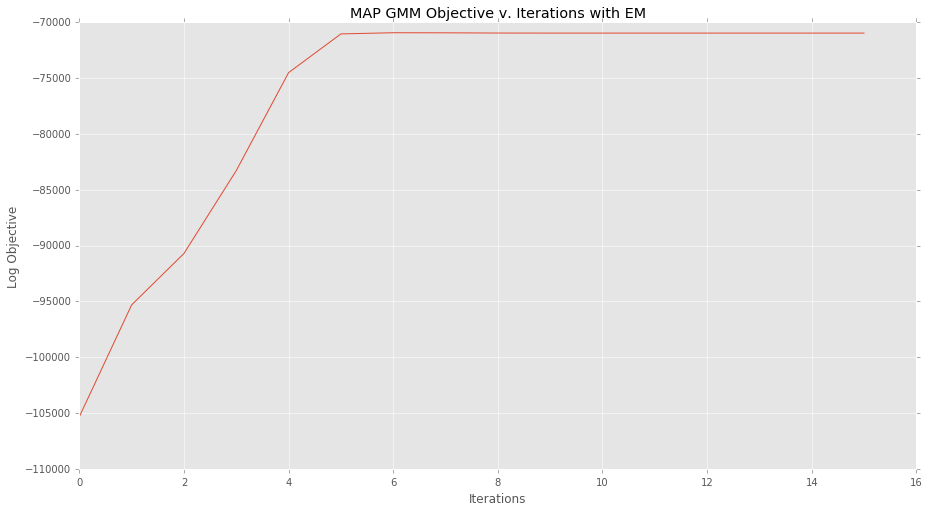
\includegraphics[scale = .5]{p3_objective.png}\\\\
\lstinputlisting[language=Python]{GaussianEM.py}

\newpage

\textbf{4 (MAP Mixture of Bernoullis)} Consider a mixture of Bernoullis with a Dirichlet prior on the mixture
weights $\pib \sim \mathrm{Dir}(\alphab)$ and a Beta prior on the mean parameter $\mu_{kj} \sim \beta(\alpha,\beta)$.
Use $\alphab=\1$ and choose an appropriate $(\alpha,\beta)$ pair for your prior (back this up).
Note that the M step for the mean is given in problem 2 (Murphy 11.3). Cluster the MNIST training dataset we used
from homework 1 (\url{http://pjreddie.com/media/files/mnist_train.csv}) using this mixture with 10 components.
Provide a convergence plot of the MAP objective
(which must monotonically increase) and plot the mean images for each component. Do the clusters roughly correspond to
different digits (back this up somehow)?

I ran into numeric problems I think, which I believe causes the slight dip in the objective function. The means also got tied together by my attempt at a numeric fix, hence the poor digit representation. The plot of the means shows that the clusters do not correspond well to the digits =(. I selected $\alpha = \beta = 1$ giving a uniform prior.

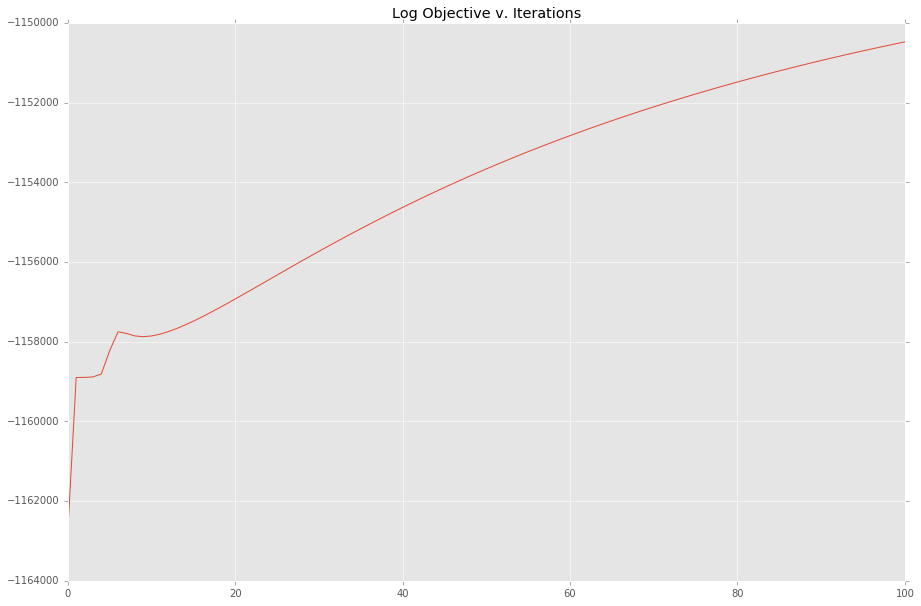
\includegraphics[scale = .5]{p4_objective_1.png}\\\\
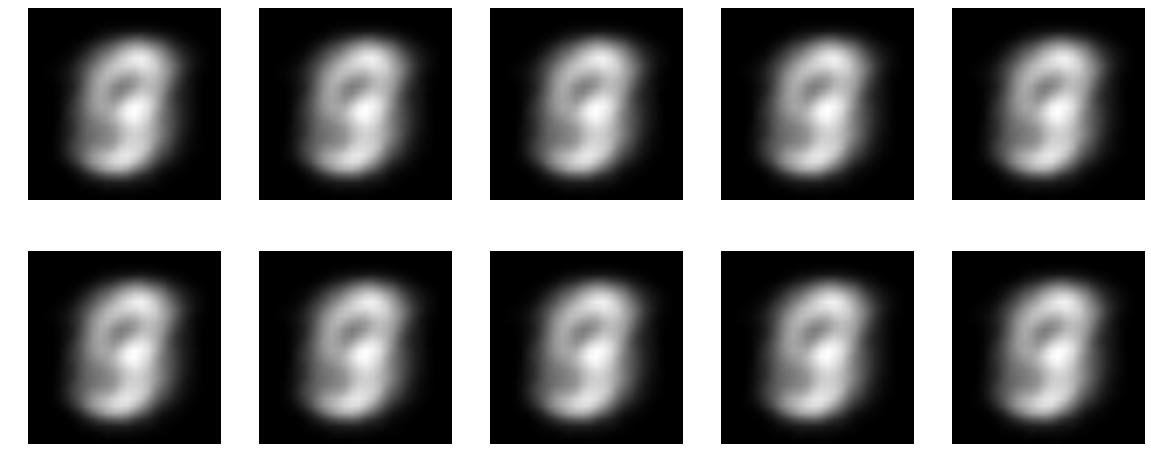
\includegraphics[scale = .25]{p4means.png}\\\\
\lstinputlisting[language=Python]{BernouliMAPwithEM.py}

\newpage

\textbf{5 (Operations Preserving Kernels)} Let $\kappa(\cdot,\cdot)$ and $\lambda(\cdot,\cdot)$ be valid positive
semi-definite (Mercer) kernels mapping from a sample space $\mathcal{S}$ to $\RR$. Let $\alpha \geq 0$ be a real number
and let $x$ and $y$ be elements of $\mathcal{S}$. Prove that
\begin{enumerate}[(a)]
    \item $\alpha\kappa(x,y)$ is a valid kernel.
    \item $\kappa(x,y) + \lambda(x,y)$ is a valid kernel.
    \item $\kappa(x,y)\lambda(x,y)$ is a valid kernel. \textit{Hint:} consider the Cholesky decomposition
        of the corresponding covariance matrix generated by the product of the kernels.
    \item $p(\kappa(x,y))$ is a valid kernel where $p(\cdot)$ is a polynomial
        with non-negative coefficients.
    \item $\exp(\kappa(x,y))$ is a valid kernel.
    \item $f(x)\kappa(x,y)f(y)$ for all $f : \mathcal{S}\to\RR$.
\end{enumerate}
To prove these, the main method would be to consider an arbitrary covariance matrix
generated by these kernels and assert that the conditions on this covariance matrix (being
symmetric and positive semi-definite) still hold.

\vspace{10mm}

\begin{enumerate}[(a)]
    \item 
        The Kernel matrix, $K_{ij} = k(x_i, x_j)$ becomes $K'_{ij} = \alpha k(x_i, x_j)$. Note a constant times a symmetric matrix is still symmetric. We can factor out the $\alpha$, so that we get $K'_{ij} = \alpha K_{ij}$. Multiplying a matrix by a constant multiplies its eigenvalues by the constant. Because $\alpha \geq 0$, the eigen values of $K'$ are still $\geq 0$, so $K' \succeq 0$, so is Mercer. 

    \item
        Note the sum of symmetric matrices is symmetric. Let $K_{ij} = k(x_i, x_j)$, $\Lambda_{ij} = \lambda(x_i, x_j)$. The sum of kernels is $K'_{ij} = k(x_i, x_j) + \lambda(x_i, x_j)$, which is an element-wise addition of $K + \Lambda$, so $K' = K + \Lambda$. The sum of positive semi-definite matrices is still positive semi-definite, so $K'$ is Mercer.

    \item
        By Mercer's theorem, $k(x, y) = \phi(x)^\T\phi(y) = \sum_i \phi(x)_i\phi(y)_i$ and $\lambda(x,y) = \sum_j \theta(x)_j\theta(y)_j$. That means $k' = k \lambda = \phi(x)^\T\phi(y) \theta(x)^\T\theta(y) = \sum_i \phi(x)_i\phi(y)_i \sum_j \theta(x)_j\theta(y)_j$. We can combine the sums by indexing over i and j, $\sum_{\forall{ij}} \phi(x)_i\phi(y)_i \theta(x)_j\theta(y)_j$. Now we can define $\phi'(x)_k = \phi(x)_i theta(x)_j$. This lets us write the sum as $\phi'(x)^\T \phi'(x) = k'$, an inner product, which, by Mercer's Theorem, means that $'k$ is Mercer.

    \item
        If we expand the polynomial, we get $p(\kappa(x,y)) = \alpha_n k(x,y)^n +\hdots+ \alpha_{1}k(x,y) + \alpha_0$. The positive power of a kernel is equivalent to multiplying kernels, which we just showed maintains validity, as does the sum. Adding a constant to a kernel ($\alpha_0$), is the same as adding a positive constant kernel, which is Mercer. Thus $p(\kappa(x,y))$ is Mercer.

    \item
        We can expand the exponent of a kernel into its Taylor series, which is a polynomial with positive constants, which we just proved is Mercer.

    \item
        We will use the same method as in part c. $k(x, y) = \phi(x)^\T\phi(y) = \sum_i \phi(x)_i\phi(y)_i$, so $k'(x,y) = f(x)\phi(x)^\T\phi(y)f(y)$. Now we define $\phi'(x) = f(x) \phi(x)$, which means we can express $k(x,y)' = \phi'(x)^\T \phi(y)$, an inner product. So by Mercer's theorem, $k'$ is a valid kernel as desired.

\end{enumerate}

\newpage

\textbf{6 (Totally Optional Extra Credit)} Prove (a), (b), and (c) from problem 5 (above) for the special
case of stationary kernels $\kappa(x,y) = \kappa(x-y)$ using Bochner's Theorem and properties of
Fourier transforms. Note that for (c) the Convolution Theorem might be helpful.

\vspace{12mm}

\begin{enumerate}[(a)]
    \item 
        We have that the Fourier transform of a Mercer kernel is $\geq 0$. The Fourier transform is a linear operator. Thus $\hat{f}[\alpha k] = \alpha \hat{f}[k] \geq 0$.
    \item
        $\hat{f}[k + \lambda] = \hat{f}[k] + \hat{f}[\lambda] \geq 0$
    \item
        The Fourier transform of a multiplication of two functions is a convolution in Fourier space. The convolution is $f * g = \int_{-\infty}^{\infty} f(\tau)g(t-\tau)$. Both kernels are positive in Fourier space, so the integral is always positive, so the kernel is valid.

\end{enumerate}

\end{document}
